\documentclass[border=6pt]{standalone}
\usepackage{amsmath,amssymb,braket}
\usepackage{tikz}
\usetikzlibrary{positioning,arrows.meta,fit,backgrounds,calc}
\begin{document}
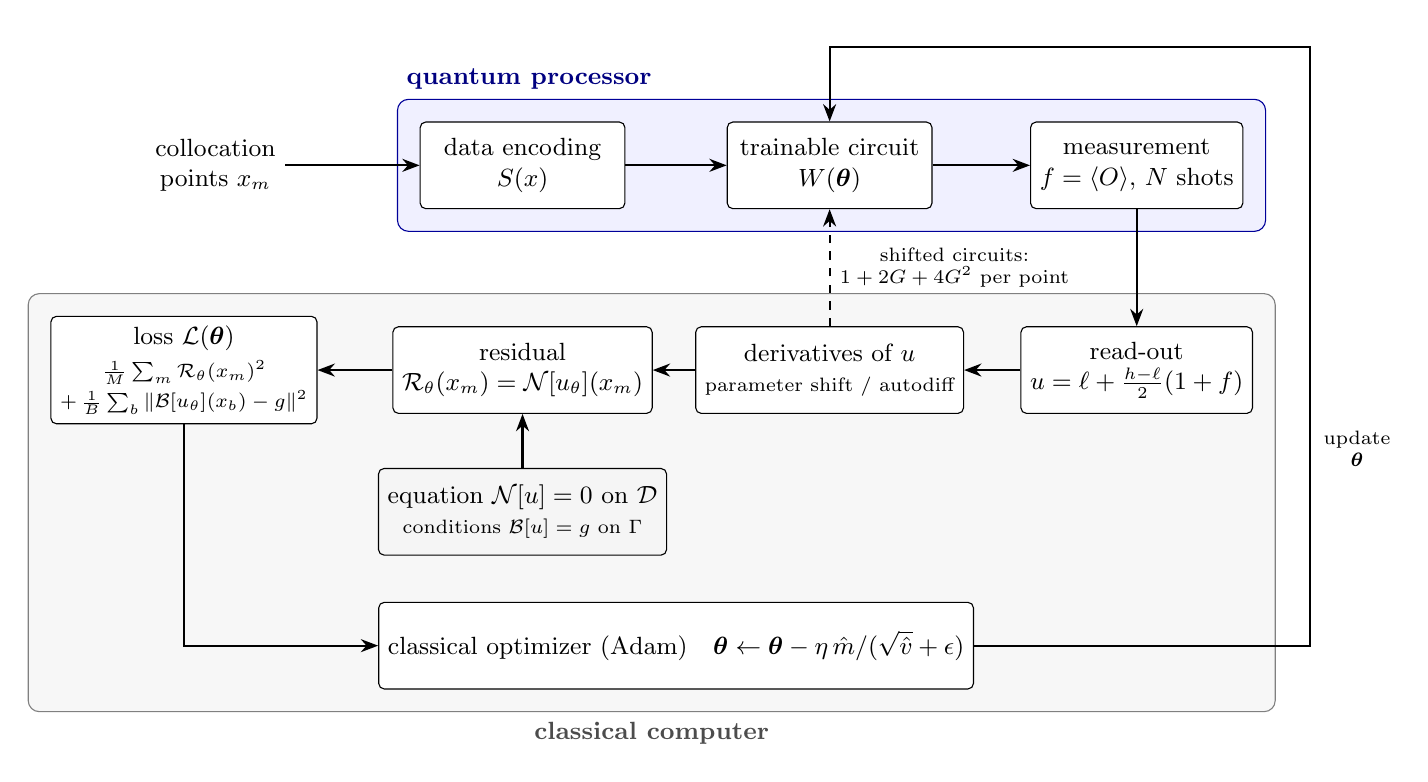
\begin{tikzpicture}[
  box/.style={draw, rounded corners=2pt, align=center, minimum height=1.1cm,
              minimum width=2.6cm, font=\small, fill=white},
  arr/.style={-{Stealth[length=2.2mm]}, thick},
  lab/.style={font=\scriptsize, align=center}]
% grid: x = 0, 3.9, 7.8, 11.7 ; rows y = 0, -2.6, -4.3, -6.0
\node[box] (enc)  at (3.9, 0)    {data encoding\\$S(x)$};
\node[box] (var)  at (7.8, 0)    {trainable circuit\\$W(\boldsymbol\theta)$};
\node[box] (meas) at (11.7, 0)   {measurement\\$f=\braket{O}$, $N$ shots};
\node[lab, font=\small] (t) at (0, 0) {collocation\\points $x_m$};

\node[box] (read) at (11.7, -2.6) {read-out\\$u=\ell+\tfrac{h-\ell}{2}(1+f)$};
\node[box] (der)  at (7.8, -2.6)  {derivatives of $u$\\{\scriptsize parameter shift / autodiff}};
\node[box] (res)  at (3.9, -2.6)  {residual\\$\mathcal R_\theta(x_m)=\mathcal N[u_\theta](x_m)$};
\node[box] (loss) at (-0.4, -2.6)    {loss $\mathcal L(\boldsymbol\theta)$\\[1pt]{\scriptsize $\frac1M\sum_m\mathcal R_\theta(x_m)^2$}\\{\scriptsize $+\,\frac1B\sum_b\|\mathcal B[u_\theta](x_b)-g\|^2$}};
\node[box, fill=black!4] (ode) at (3.9, -4.4) {equation $\mathcal N[u]=0$ on $\mathcal D$\\{\scriptsize conditions $\mathcal B[u]=g$ on $\Gamma$}};
\node[box, minimum width=6cm] (opt) at (5.85, -6.1)
      {classical optimizer (Adam)\quad $\boldsymbol\theta\leftarrow\boldsymbol\theta-\eta\,\hat m/(\sqrt{\hat v}+\epsilon)$};

\draw[arr] (t) -- (enc);
\draw[arr] (enc) -- (var);
\draw[arr] (var) -- (meas);
\draw[arr] (meas) -- (read);
\draw[arr] (read) -- (der);
\draw[arr] (der) -- (res);
\draw[arr] (res) -- (loss);
\draw[arr] (ode) -- (res);
\draw[arr] (loss.south) |- (opt.west);
\draw[arr] (opt.east) -| (13.9, -1.3) |- (7.8, 1.5) -- (var.north)
      node[pos=0.0, above, lab] {};
\node[lab, anchor=west] at (13.95, -3.6) {update\\$\boldsymbol\theta$};
\draw[arr, dashed] (der.north) -- (var.south)
      node[lab, pos=0.5, right] {shifted circuits:\\$1+2G+4G^2$ per point};

\begin{scope}[on background layer]
  \node[draw=blue!60!black, fill=blue!6, rounded corners=4pt, inner sep=8pt,
        fit=(enc)(var)(meas), label={[font=\small\bfseries, text=blue!50!black, anchor=south west]north west:quantum processor}] {};
  \node[draw=black!50, fill=black!3, rounded corners=4pt, inner sep=8pt,
        fit=(read)(der)(res)(loss)(ode)(opt), label={[font=\small\bfseries, text=black!70]below:classical computer}] {};
\end{scope}
\end{tikzpicture}
\end{document}
